\documentclass{beamer}
\usepackage{tikz}
\usepackage{multimedia}
\usepackage{hyperref}
\usepackage{polski}
\usepackage[utf8]{inputenc}
\usepackage[T1]{fontenc}
\usepackage{color}
\usepackage{amsthm}
\usepackage{graphicx}
\usepackage{makecell}
\usepackage{booktabs}
\usetheme{Warsaw}


\title{Rozpoznawanie tablic rejestracyjnych pojazdów na obrazach z kamery samochodowej}
\author{Marcin Łykowski}

\begin{document}
    \begin{frame}
        \maketitle
        \centering
        Promotor: dr hab.inż. Przemysław Klęsk
    \end{frame}


    \section{Cel i zakres pracy}
    \begin{frame}
        \frametitle{Cel i zakres pracy}
        Celem niniejszej pracy jest przedstawienie tematyki rozpoznawania tablic rejestracyjnych.
        W zakres pracy wchodzą:
        \begin{itemize}
            \item omówienie wybranych algorytmów z zakresu przetwarzania obrazów i uczenia maszynowego, potrzebnych do realizacji postawionego zadania,
            \item przygotowania odpowiedniego materiału (sekwencje wideo) na potrzeby uczenia maszynowego i testowania,
            \item przedstawienie ostatecznego schematu algorytmicznego dla całego procesu,
            \item przeprowadzenie eksperymentów, pomiary dokładności i czasów wykonania, wnioski końcowe.
        \end{itemize}
    \end{frame}


    \section{Wprowadzenie}

    \begin{frame}
        \frametitle{Rozpoznawanie tablic rejestracyjnych}
        \begin{itemize}
            \item \textbf{Detekcja} --- określenie położenia tablicy rejestracyjnej w analizowanym obrazie.
            \item \textbf{Segmentacja} --- wyodrębnienie pojedynczych znaków na fragmencie obrazu ze zlokalizowaną tablicą.
            \item \textbf{Identyfikacja} --- rozpoznanie każdego ze znaków i przedstawienie ich w formie tekstowej, którą można później wykorzystać do dalszych działań w zależności od przeznaczenia systemu.
        \end{itemize}
    \end{frame}

    \begin{frame}
        \frametitle{Rozpoznawanie tablic rejestracyjnych}
        \begin{figure}
            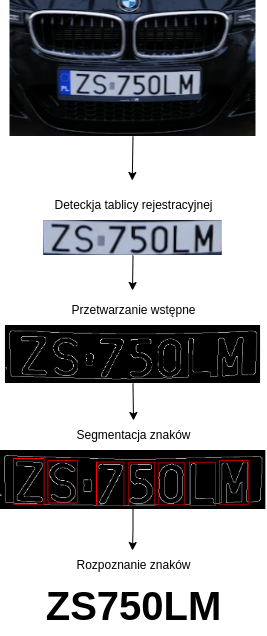
\includegraphics[scale=0.3]{../WIZUT-Dyplom-styl/Pictures/schemat_lpr}
        \end{figure}
    \end{frame}

    \begin{frame}
        \frametitle{Potencjalne trudności}
        \begin{itemize}
            \item zajmowanie niewielkiego obszaru na zdjęciu przez tablicę rejestracyjną
            \item istnienie ogromnej liczby formatów tablic rejestracyjnych (w zależności od kraju rejestracji lub rodzaju pojazdu)
            \item słabe oświetlenie, rozmazany obraz, refleksy świetlne
            \item ruch pojazdu, zabrudzone tablice
        \end{itemize}
    \end{frame}


    \section{Opracowaine zbioru uczącego}

    \begin{frame}
        \frametitle{Przykładowe klatki wideo z kamery samochodowej}
        \begin{figure}
            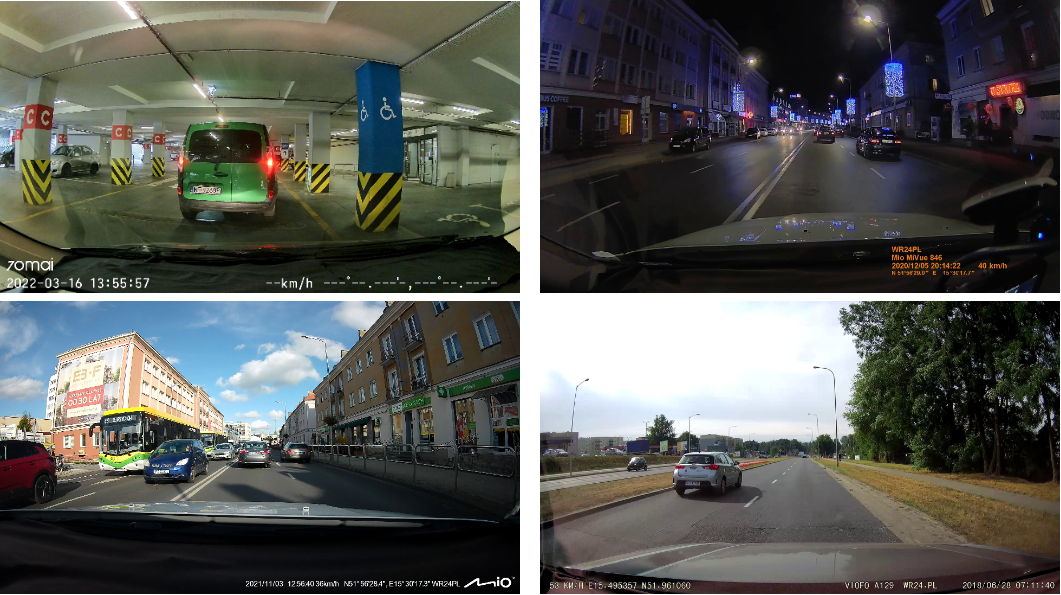
\includegraphics[scale=0.3]{../WIZUT-Dyplom-styl/Pictures/captured_frames}
        \end{figure}
    \end{frame}

    \begin{frame}
        \frametitle{Szczegóły zbioru uczącego}
        \begin{table}[h]
            \centering
            \scalebox{0.9}{
                \begin{tabular}{l l l}
                    \toprule
                    \textbf{Parametr}                      & \textbf{Wartość}                                     \\
                    \midrule
                    Liczba zdjęć                           & 10985                                                \\
                    Format zdjęć                           & JPG                                                  \\
                    Liczba zdjęć zawierających tablice     & 5248                                                 \\
                    Ogółem liczba tablic                   & 10301                                                \\
                    Zakres liczby tablic na jednym zdjęciu & 0--6                                                 \\
                    Średnia wysokość próbki                & 38px                                                 \\
                    Średnia szerokość próbki               & 91px                                                 \\
                    Maksymalne rozmiary próbki             & 378$\times$136px                                     \\
                    Minimalne rozmiary próbki              & 15$\times$11px                                       \\
                    Rozdzielczości zdjęć                   & 1920$\times$1080, 2560$\times$1440, 3840$\times$2160 \\
                    Liczba klatek na sekundę               & 30 kl/s, 60 kl/s                                     \\
                    \bottomrule
                \end{tabular}}
            \label{tab:tab_data_set_characteristics}
        \end{table}
    \end{frame}


    \section{Opracowany algorytm}

    \begin{frame}
        \frametitle{Opracowany algorytm}
        Do detekcji użyto skanowania obrazu oknem przesuwnym i klasyfikowanie na podstawie cech Haara za pomocą algorytmu RealBoost.
        Jako słaby klasyfikator wykorzystano algorytm koszykowania wartości funkcji logit.
        Rozpoznane fragmenty obrazu zawierające tablice poddano operacjom morfologicznym.
        Z przetworzonych obrazów segmentowano znaki tablicy rejestracyjnej.
        Do rozpoznania znaków użyto biblioteki Tesseract opartej o rekurencyjne sieci neuronowe LSTM\@.
        \begin{figure}
            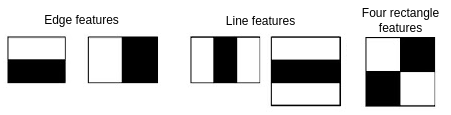
\includegraphics[scale=0.3]{../WIZUT-Dyplom-styl/Pictures/haar_feats}
        \end{figure}
    \end{frame}

    \begin{frame}
        \frametitle{Opracowany algorytm}
        \begin{figure}
            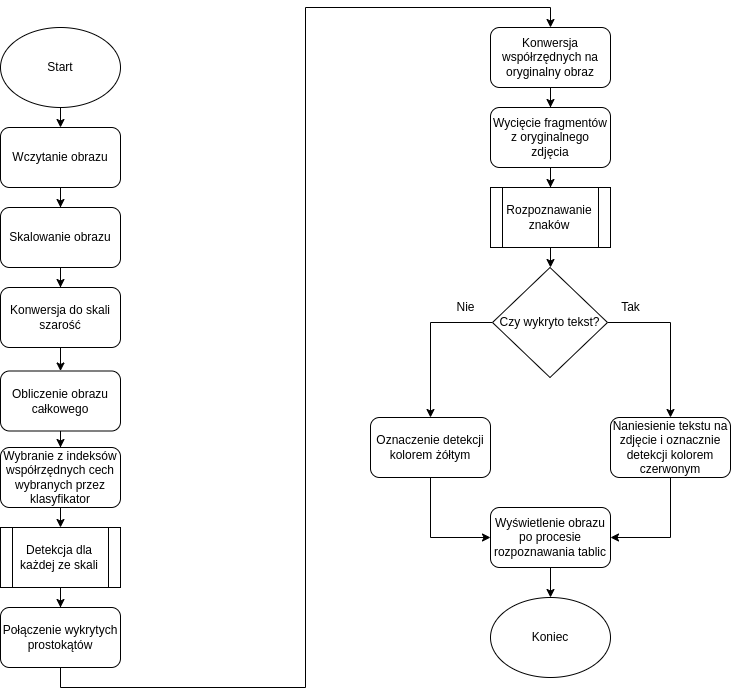
\includegraphics[scale=0.25]{../WIZUT-Dyplom-styl/Pictures/main_alg_scaled}
        \end{figure}
    \end{frame}

    \begin{frame}
        \frametitle{Algorytm detekcji}
        \begin{figure}
            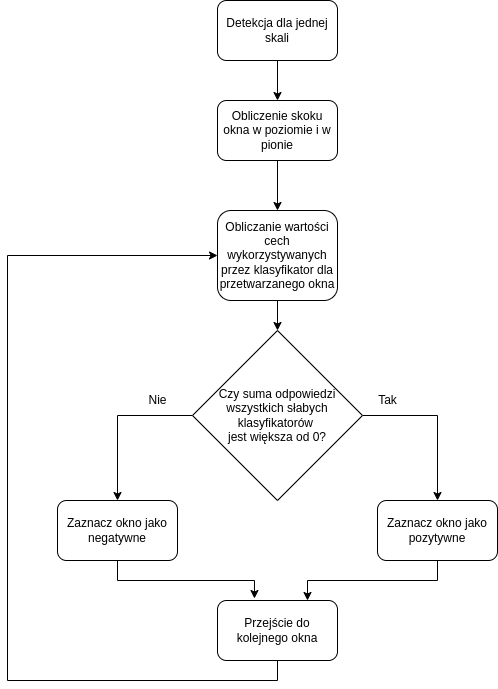
\includegraphics[scale=0.2]{../WIZUT-Dyplom-styl/Pictures/detection_alg}
        \end{figure}
    \end{frame}

    \begin{frame}
        \frametitle{Wynik detekcji}
        \begin{figure}
            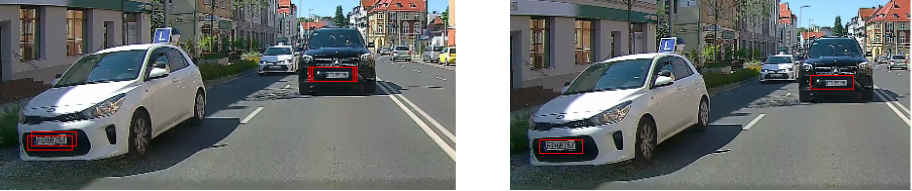
\includegraphics[scale=0.3]{../WIZUT-Dyplom-styl/Pictures/non_max_supression}
        \end{figure}
    \end{frame}

    \begin{frame}
        \frametitle{Algorytm segmentacji}
        \begin{figure}
            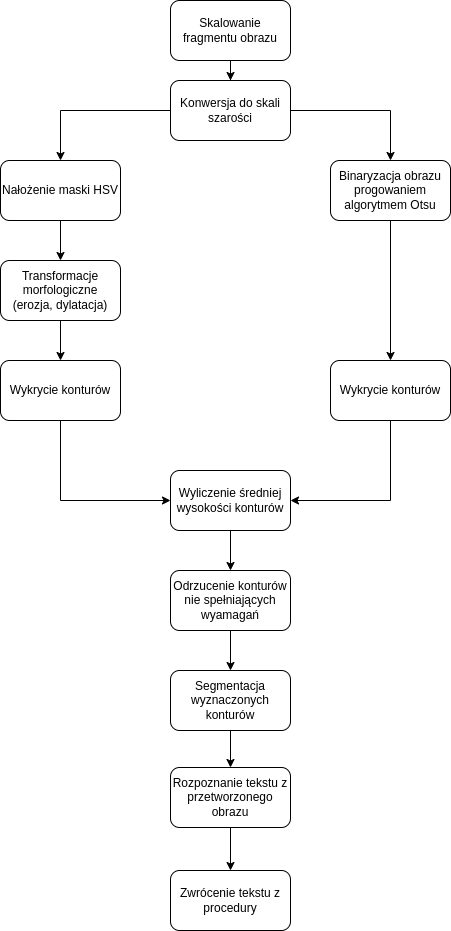
\includegraphics[scale=0.2]{../WIZUT-Dyplom-styl/Pictures/characters_alg}
        \end{figure}
    \end{frame}

    \begin{frame}
        \frametitle{Wynik segmentacji}
        \begin{figure}
            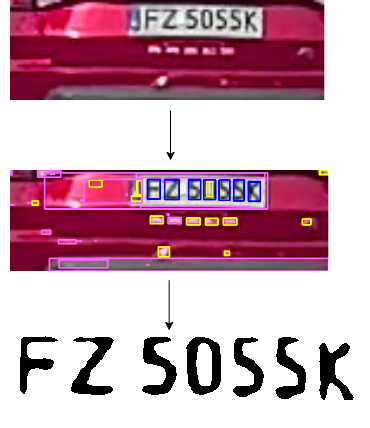
\includegraphics[scale=0.3]{../WIZUT-Dyplom-styl/Pictures/segmentation}
        \end{figure}
    \end{frame}


    \section{Wyniki badań}

    \begin{frame}
        \frametitle{Wyniki badań}
        \begin{table}[h]
            \centering
            \label{tab:accuracy_clf}
            \scalebox{0.8}{
                \begin{tabular}{c c c c c c}
                    \toprule
                    \textbf{\thead{Liczba \\cech}} & \textbf{\thead{Liczba  \\słabych \\klasyfikatorów}} & \textbf{\thead{Liczba \\koszyków}} & \textbf{\thead{Dokładność \\klasyfikatora}} & \textbf{\thead{Dokładność \\klasyfikatora dla \\próbek pozytywnych}} & \textbf{\thead{Dokładność \\klasyfikatora dla \\próbek negatywnych}} \\
                    \midrule
                    2205 & 32 & 8 & 99.70\% & 75.15\% & 99.94\% \\
                    2205 & 64 & 8 & 99.77\% & 82.24\% & 99.94\% \\
                    2205 & 256 & 8 & 99.87\% & 91.12\% & 99.96\% \\
                    \bottomrule
                \end{tabular}}
        \end{table}
    \end{frame}

    \begin{frame}
        \frametitle{Wyniki badań}
        \begin{figure}
            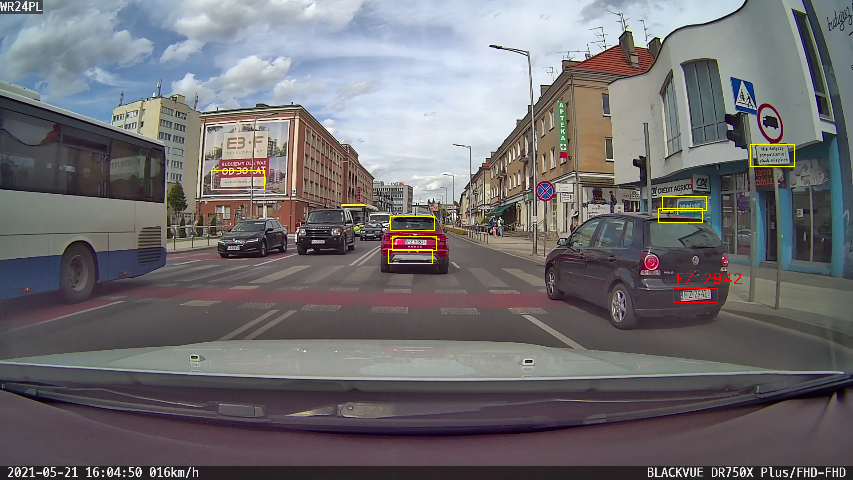
\includegraphics[scale=0.3]{../WIZUT-Dyplom-styl/Pictures/tablica_rozpoznana}
        \end{figure}
    \end{frame}

    \begin{frame}
        \frametitle{Wyniki badań}
        \begin{figure}
            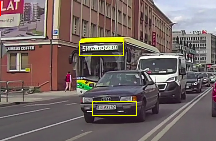
\includegraphics[scale=0.6]{../WIZUT-Dyplom-styl/Pictures/autobus}
        \end{figure}
    \end{frame}

    \begin{frame}
        \frametitle{Wyniki badań}
        \begin{figure}
            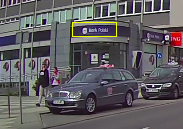
\includegraphics[scale=0.6]{../WIZUT-Dyplom-styl/Pictures/bank}
        \end{figure}
    \end{frame}

    \begin{frame}
        \frametitle{Wyniki badań}
        \begin{figure}
            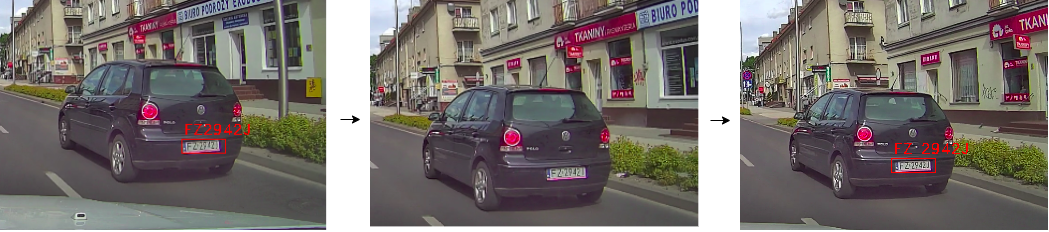
\includegraphics[scale=0.3]{../WIZUT-Dyplom-styl/Pictures/same_car}
        \end{figure}
    \end{frame}

    \begin{frame}
        \frametitle{Wyniki badań}
        \begin{figure}
            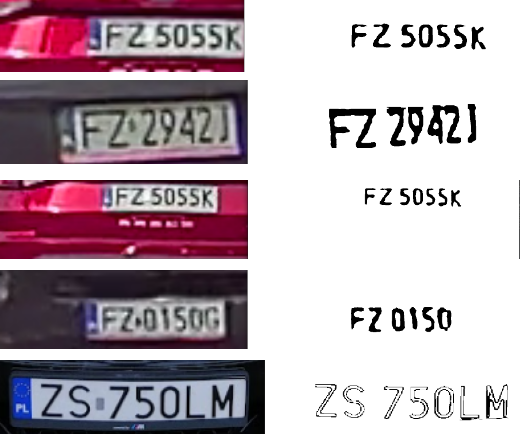
\includegraphics[scale=0.3]{../WIZUT-Dyplom-styl/Pictures/plates}
        \end{figure}
    \end{frame}

    \begin{frame}
        \frametitle{Wydajność czasowa systemu}
        \begin{table}[h]
            \centering
            \label{tab:performance}
            \scalebox{0.9}{
                \begin{tabular}{c c c c c c}
                    \toprule
                    \textbf{\thead{Liczba \\cech}} & \textbf{\thead{Liczba  \\unikalnych cech \\użytych przez \\ klasyfikator}} & \textbf{\thead{Liczba \\okien}} & \textbf{\thead{Czas \\detekcji}} & \textbf{\thead{Czas \\rozpoznawania \\jednej tablicy}} & \textbf{\thead{Czas przetwarzania \\jednego okna}} \\
                    \midrule
                    2205 & 32 & 39188 & 0.68s & 0.11s & 0.4ms \\
                    2205 & 64 & 39188 & 0.91s & 0.12s & 0.9ms \\
                    2205 & 256 & 39188 & 2.24s & 0.11s & 1.1ms \\
                    \bottomrule
                \end{tabular}}
        \end{table}
    \end{frame}

    \begin{frame}
        \frametitle{Propozycje udoskonalenia algorytmu}
        \begin{itemize}
            \item dołożenie do zbioru uczącego negatywnych okien, które obecnie klasyfikator wykrywa błędnie, jako pozytywne
            \item użycie więcej niż jednego klasyfikatora do detekcji obiektów
            \item użycie kompilowanego języka w celu zwiększenia wydajności
            \item nauczenie sieci neuronowej zbiorem znaków pochodzących z tablic rejestracyjnych
        \end{itemize}

%        Jednym z pomysłów na udoskonalenie modułu detekcji jest dołożenie do zbioru uczącego negatywnych okien, które obecnie klasyfikator wykrywa błędnie, jako pozytywne.
%        Jest prawdopodobnym, że ponownie nauczony klasyfikator charakteryzowałby się wyższą dokładnością detekcji.
%        Innym pomysłem, który mógłby poprawić wydajność oraz jakość detekcji jest użycie więcej niż jednego klasyfikatora do detekcji obiektów.
%        W pierwszej kolejności jeden klasyfikator klasyfikowałby okna zawierający samochody.
%        Tak działający klasyfikator działałby szybciej, ponieważ rozmiar okna w procedurze skanującej byłby większy.
%        Wynika to z faktu, że samochód zajmuje większy obraz na zdjęciu niż jego tablica rejestracyjna.
%        Następnie na wykrytych fragmentach należałoby wykryć tablice rejestracyjne.
%        W rezultacie liczba okien poddawanych procedurze predykcji mogłaby być mniejsza niż w oryginalnym rozwiązaniu.
%        Aby zwiększyć wydajność rozwiązania, możliwe jest również zaimplementowanie programu w silnie typowanym, kompilowanym języku, np.\ C++.
%
%        W celu poprawienia jakości rozpoznawania znaków, możliwe jest nauczenie sieci neuronowej biblioteki Tesseract zbiorem znaków z tablic rejestracyjnych.
%        Biblioteka domyślnie wyuczona jest na zbiorach znaków pochodzących z różnego rodzaju tekstów drukowanych, tj.\ książki lub dokumenty.
%        Podczas przygotowywania zbioru uczącego, szczególną uwagę należałoby przykuć do przygotowania znaków, które nie mają idealnych konturów.
%        Ma to na celu zapewnienie przykładów uczących maksymalnie zbliżonych do próbek w realnym środowisku pracy.
    \end{frame}


    \section{}
    \begin{frame}
        \begin{center}
        {\Huge Dziękuję za uwagę}
        \end{center}
    \end{frame}

\end{document}
